\section{Check for Understanding: The Egg Throw}

\begin{overview}

	\textbf{Overview:} In this section, we'll attempt to explain a new phenomenon (another party trick, if you will) with the models we've accumulated, so far.
	
\end{overview}

\textbf{Consider the following two phenomena:}

\begin{enumerate}
	\item Egg thrown at velocity $\vec{v}$ at a wall that stands motionless with respect to the earth.
	
	\item Egg thrown at velocity $\vec{v}$ at a bed sheet that is held by two people standing motionless with respect to the earth.
\end{enumerate}

\noindent For both cases, consider the following interval:

\begin{center}
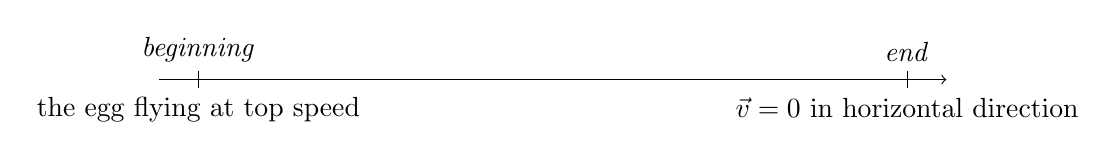
\begin{tikzpicture}
    % draw horizontal line   
    \draw[->] (0,0) -- (10,0);

    % draw vertical lines
    \foreach \x in {0.5,9.5}
      \draw (\x cm,3pt) -- (\x cm,-3pt);

    % draw nodes
    \draw (0.5,0) node[below=3pt] {the egg flying at top speed} node[above=3pt] {\emph{beginning}};
    \draw (9.5,0) node[below=3pt] {$\vec{v}=0$ in horizontal direction} node[above=3pt] {\emph{end}};
\end{tikzpicture}
\end{center}

\noindent\textbf{Make sure everyone in your group fully understands the ideas behind each question or part below before going on to the next part.}

\begin{enumerate}
	\item In your small groups, predict if the egg will or will not break in either case.
	\item Use your intuition to think about what factors determine whether the egg will break or not. List these factors on your group's board.
	\item Use ideas, models, language, and/or equations from this class to explain why these factors are important. 
	
\WCD
\end{enumerate}

\noindent\textbf{Now, go do it!} You will investigate the egg throw cases together as a class.

\begin{itemize}
	\item Come up with a logical argument for why the egg does or does not break in either case.
	\item Write out your argument as you might on a quiz.
	\item Use physics ideas, models, words, and/or equations from class to explain your reasoning.
\end{itemize}

\WCD